% !TEX program = pdflatex
% Build from the repository root with:
%   python3 /Users/entropy/.codex/plugins/cache/openai-bundled/latex/0.2.4/scripts/compile_latex.py \
%     /Users/entropy/Git/GraphNAMLSS/paper/main.tex
\documentclass[11pt]{article}

\usepackage[T1]{fontenc}
\usepackage[utf8]{inputenc}
\usepackage{lmodern}
\usepackage{microtype}
\usepackage[a4paper,margin=25mm]{geometry}
\usepackage{amsmath,amssymb,mathtools,bm}
\usepackage{booktabs,tabularx,multirow}
\usepackage{siunitx}
\usepackage{xcolor}
\usepackage{graphicx}
\usepackage{subcaption}
\usepackage{tikz}
\usepackage{pgfplots}
\usepackage[round,authoryear]{natbib}
\usepackage[colorlinks=true,allcolors=blue!55!black]{hyperref}
\usepackage[nameinlink,noabbrev]{cleveref}

\usetikzlibrary{arrows.meta,backgrounds,calc,fit,positioning}
\pgfplotsset{compat=1.18}

\definecolor{localblue}{HTML}{276FBF}
\definecolor{graphorange}{HTML}{E07A1F}
\definecolor{locationgreen}{HTML}{2A9D8F}
\definecolor{scalered}{HTML}{D1495B}
\definecolor{ink}{HTML}{243447}
\definecolor{softgray}{HTML}{F2F4F7}
\definecolor{placeholdergray}{HTML}{6B7280}

\newcommand{\method}{GraphNAMLSS}
\newcommand{\datasetA}{METR-LA}
\newcommand{\datasetB}{PEMS-BAY}
\newcommand{\placeholder}[1]{\textcolor{placeholdergray}{\textit{[#1]}}}
\newcommand{\trainset}{\mathcal{T}_{\mathrm{train}}}
\newcommand{\graph}{\mathcal{G}}
\newcommand{\neighbors}{\mathcal{N}}
\newcommand{\softplus}{\operatorname{softplus}}
\newcommand{\crps}{\operatorname{CRPS}}
\newcommand{\nll}{\operatorname{NLL}}
\newcommand{\E}{\mathbb{E}}
\newcommand{\R}{\mathbb{R}}

\title{\method: Interpretable Distributional Regression on Graphs\\
with an Application to Traffic Speed Forecasting}
\author{%
  \placeholder{Author names}\\
  \small \placeholder{Affiliations}\\
  \small \texttt{\placeholder{corresponding.author@example.org}}
}
\date{}

\begin{document}
\maketitle

\begin{abstract}
\method{} combines parameter-wise neural additive predictors with graph-derived
contributions. We formulate the method for Gaussian location--scale regression
and evaluate it on 15-minute-ahead traffic speed forecasting.
\placeholder{Insert one sentence with the principal numerical result only after
the real-data merit probe is complete.}
\end{abstract}

\section{Introduction}
\label{sec:introduction}

Distributional regression predicts a conditional distribution rather than only
its mean. Graph neural networks exploit relational structure, but their
distributional heads are usually difficult to decompose. We propose \method{} to
separate local covariate effects from parameter-specific graph effects.

\paragraph{Contributions.}
The paper evaluates: (i) graph information beyond a local NAMLSS predictor,
(ii) distinct graph effects on location and scale, and (iii) the accuracy--
interpretability trade-off against a non-additive distributional GNN.

\section{Related work}
\label{sec:related}

GAMLSS models multiple parameters of a response distribution
\citep{rigby2005gamlss}. Neural additive models retain feature-wise shape
functions \citep{agarwal2021nam}, and NAMLSS extends this idea beyond the
conditional mean \citep{thielmann2023namlss}. GraphSAGE provides a simple
neighborhood aggregation mechanism \citep{hamilton2017graphsage}. Traffic
forecasting models such as DCRNN and Graph WaveNet demonstrate the value of road
network structure on \datasetA{} and \datasetB{}
\citep{li2018dcrnn,wu2019graphwavenet}. \method{} targets the remaining
intersection: decomposable, parameter-specific distributional graph regression.

\section{Problem formulation}
\label{sec:problem}

Let $\graph=(\mathcal{V},\mathcal{E},\bm{A})$ be a directed weighted graph with
nodes $i\in\mathcal{V}$ and edge weights $a_{ji}\geq 0$. At time $t$, node $i$
has local covariates $\bm{x}_{it}\in\R^p$, graph-stream covariates
$\bm{z}_{it}\in\R^q$, and response $y_{it}$. For a $K$-parameter family,
\begin{equation}
  Y_{it}\mid \bm{x}_{it},\bm{Z}_t,\graph
  \sim \mathcal{D}\!\left(
    \theta_{1,it},\ldots,\theta_{K,it}
  \right),
  \qquad
  \theta_{k,it}=g_k^{-1}(\eta_{k,it}).
  \label{eq:distributional-regression}
\end{equation}
The objective is to improve the predictive distribution using graph context
while keeping the contribution to each $\eta_{k,it}$ inspectable.

\section{\method}
\label{sec:method}

\subsection{Centered local additive predictor}

For parameter $k$, feature $j$ has a learned shape function $f_{kj}$. Its
training-reference-centered contribution is
\begin{align}
  c_{kj}
    &= \frac{1}{|\trainset|}
       \sum_{(i,t)\in\trainset} f_{kj}(x_{j,it}),
  &
  \widetilde f_{kj}(x_{j,it})
    &= f_{kj}(x_{j,it})-c_{kj},                                      \label{eq:local-centering}\\
  \eta^{\mathrm{local}}_{k,it}
    &= \beta_{k0}+\sum_{j=1}^{p}\widetilde f_{kj}(x_{j,it}).          \label{eq:local-predictor}
\end{align}
Reference centering fixes the intercept interpretation and prevents evaluation
batches from changing the decomposition.

\subsection{Neighbor-focused graph encoder}

Set $\bm{h}^{(0)}_{it}=\bm{z}_{it}$. A weighted GraphSAGE-style layer computes
\begin{align}
  \bm{m}^{(\ell)}_{it}
    &=
    \frac{\sum_{j\in\neighbors(i)}
      a_{ji}\bm{h}^{(\ell-1)}_{jt}}
    {\max\!\left(\sum_{j\in\neighbors(i)}a_{ji},\,\epsilon_A\right)},
                                                                    \label{eq:aggregation}\\
  \bm{h}^{(\ell)}_{it}
    &= \rho\!\left(
      \bm{W}^{(\ell)}
      [\,\bm{h}^{(\ell-1)}_{it}\Vert\bm{m}^{(\ell)}_{it}\,]
      +\bm{b}^{(\ell)}
    \right), \qquad \ell=1,\ldots,L,                                \label{eq:graphsage}
\end{align}
where $\rho$ is ReLU. In the neighbor-focused variant, $\bm{z}_{it}$ contains
traffic lags and missingness indicators but no calendar features.

\subsection{Parameter-specific centered graph contribution}

A shared encoder feeds a separate linear head for each distributional
parameter:
\begin{align}
  r_{k,it}
    &= \bm{w}_k^\top\bm{h}^{(L)}_{it}+b_k,                            \label{eq:graph-head}\\
  \bar r_k
    &= \frac{1}{|\trainset|}\sum_{(i,t)\in\trainset}r_{k,it},
  &
  \widetilde r_{k,it}
    &= r_{k,it}-\bar r_k,                                            \label{eq:graph-centering}\\
  \eta_{k,it}
    &= \eta^{\mathrm{local}}_{k,it}
       +\alpha_k\widetilde r_{k,it}.                                 \label{eq:graphnamlss}
\end{align}
The scalar $\alpha_k$ is a graph-contribution gate. The observable
parameter-specific graph effect is the product
$\alpha_k\widetilde r_{k,it}$; $\alpha_k$ alone is not an effect size and has
no causal interpretation.

\begin{figure}[t]
  \centering
  \resizebox{\linewidth}{!}{%
  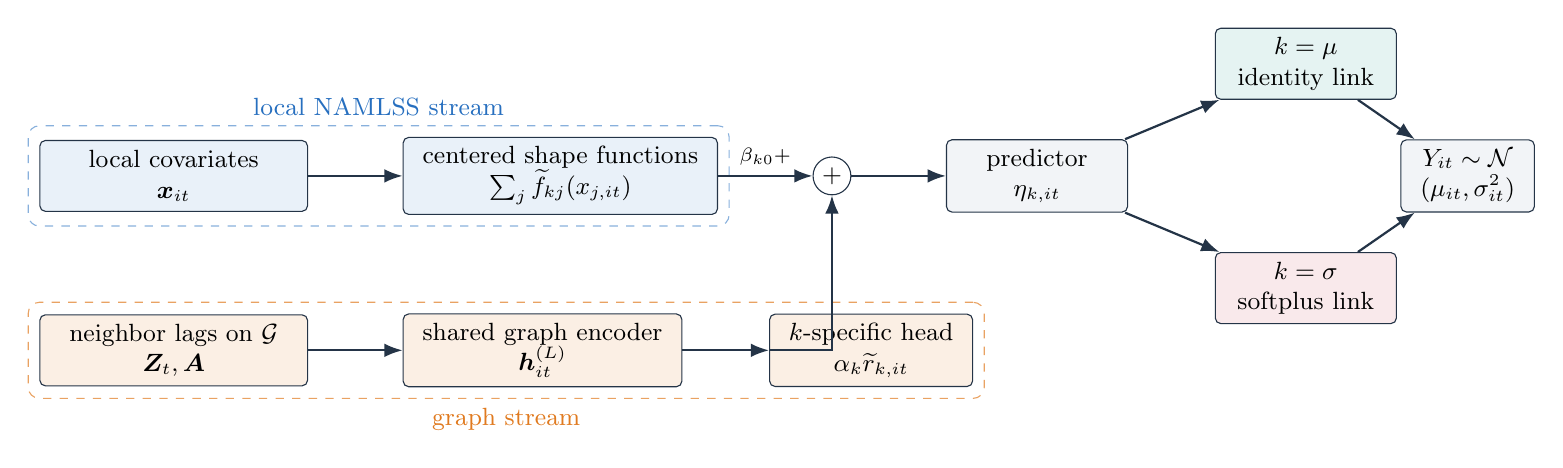
\begin{tikzpicture}[
    font=\small,
    >=Latex,
    box/.style={draw=ink, rounded corners=2pt, align=center,
      minimum height=9mm, inner xsep=7pt, fill=white},
    stream/.style={box, minimum width=34mm},
    head/.style={box, minimum width=23mm},
    arrow/.style={->, thick, draw=ink},
    add/.style={circle, draw=ink, fill=white, inner sep=1.5pt},
  ]
    \node[stream, fill=localblue!10] (x) {local covariates\\$\bm{x}_{it}$};
    \node[stream, fill=localblue!10, right=12mm of x] (shape)
      {centered shape functions\\$\sum_j\widetilde f_{kj}(x_{j,it})$};
    \node[stream, fill=graphorange!12, below=13mm of x] (z)
      {neighbor lags on $\graph$\\$\bm{Z}_t,\bm{A}$};
    \node[stream, fill=graphorange!12, right=12mm of z] (enc)
      {shared graph encoder\\$\bm{h}^{(L)}_{it}$};
    \node[head, fill=graphorange!12, right=11mm of enc] (ghead)
      {$k$-specific head\\$\alpha_k\widetilde r_{k,it}$};
    \node[add, right=12mm of shape] (plus) {$+$};
    \node[head, fill=softgray, right=12mm of plus] (eta)
      {predictor\\$\eta_{k,it}$};
    \node[head, fill=locationgreen!12, above right=5mm and 11mm of eta] (mu)
      {$k=\mu$\\identity link};
    \node[head, fill=scalered!12, below right=5mm and 11mm of eta] (sigma)
      {$k=\sigma$\\softplus link};
    \node[box, right=12mm of $(mu)!0.5!(sigma)$, fill=softgray] (dist)
      {$Y_{it}\sim\mathcal{N}$\\$(\mu_{it},\sigma_{it}^2)$};

    \draw[arrow] (x) -- (shape);
    \draw[arrow] (z) -- (enc);
    \draw[arrow] (enc) -- (ghead);
    \draw[arrow] (shape) -- node[above, font=\scriptsize] {$\beta_{k0}+$} (plus);
    \draw[arrow] (ghead) -| (plus);
    \draw[arrow] (plus) -- (eta);
    \draw[arrow] (eta) -- (mu);
    \draw[arrow] (eta) -- (sigma);
    \draw[arrow] (mu) -- (dist);
    \draw[arrow] (sigma) -- (dist);

    \begin{scope}[on background layer]
      \node[draw=localblue!55, dashed, rounded corners=4pt, fit=(x)(shape),
        inner sep=4pt, label={[text=localblue]above:local NAMLSS stream}] {};
      \node[draw=graphorange!70, dashed, rounded corners=4pt, fit=(z)(enc)(ghead),
        inner sep=4pt, label={[text=graphorange]below:graph stream}] {};
    \end{scope}
  \end{tikzpicture}%
  }
  \caption{Parameter-wise decomposition of \method. The encoder may be shared,
  but the graph head and gate are specific to each distributional parameter.}
  \label{fig:architecture}
\end{figure}

\subsection{Gaussian location--scale specialization}

For the traffic application,
\begin{equation}
  Y_{it}\mid\bm{x}_{it},\bm{Z}_t,\graph
  \sim\mathcal{N}(\mu_{it},\sigma_{it}^2),
  \qquad
  \mu_{it}=\eta_{\mu,it},
  \qquad
  \sigma_{it}=\softplus(\eta_{\sigma,it})+\epsilon_\sigma.
  \label{eq:gaussian-links}
\end{equation}
With observation mask $o_{it}\in\{0,1\}$, the training loss is
\begin{equation}
  \mathcal{L}_{\mathrm{NLL}}
  =
  \frac{1}{\sum_{(i,t)\in\trainset}o_{it}}
  \sum_{(i,t)\in\trainset}o_{it}
  \left[
    \frac{1}{2}\log(2\pi)
    +\log\sigma_{it}
    +\frac{(y_{it}-\mu_{it})^2}{2\sigma_{it}^2}
  \right].
  \label{eq:nll}
\end{equation}
All preprocessing statistics and the centering constants in
\cref{eq:local-centering,eq:graph-centering} are estimated on the training
partition only.

\subsection{Model-family variants}

The full family crosses representation sharing, injection strategy, and
self-feature access (\cref{tab:matrix}). For graph-aware shape functions, let
$s_{j,it}$ summarize feature $j$ in the neighborhood. The alternative predictor
is
\begin{equation}
  \eta_{k,it}
  =
  \beta_{k0}
  +\sum_{j=1}^{p}\widetilde f^{\mathrm{local}}_{kj}(x_{j,it})
  +\sum_{j=1}^{p}\widetilde f^{\mathrm{context}}_{kj}
    (x_{j,it},s_{j,it}).
  \label{eq:context-shape}
\end{equation}
The context terms require their own centering constraint so that they cannot
absorb the local main effects.

\begin{table}[t]
  \centering
  \caption{Primary $2\times2\times2$ experiment matrix. The bold row is the
  tracer-bullet model.}
  \label{tab:matrix}
  \begin{tabular}{lll}
    \toprule
    Graph representation & Graph injection & Self-feature access\\
    \midrule
    \textbf{Shared} & \textbf{Additive contribution} & \textbf{Neighbor-focused}\\
    Shared & Additive contribution & Self-inclusive\\
    Shared & Graph-aware shapes & Neighbor-focused\\
    Shared & Graph-aware shapes & Self-inclusive\\
    Per-parameter & Additive contribution & Neighbor-focused\\
    Per-parameter & Additive contribution & Self-inclusive\\
    Per-parameter & Graph-aware shapes & Neighbor-focused\\
    Per-parameter & Graph-aware shapes & Self-inclusive\\
    \bottomrule
  \end{tabular}
\end{table}

\section{Traffic-network application}
\label{sec:application}

\subsection{Forecasting task}

For five-minute observations, the target is the speed three steps ahead,
\begin{equation}
  y_{it}=v_{i,t+3}.
  \label{eq:traffic-target}
\end{equation}
Local features contain current speed, lags at 5, 10, 15, 30, and 60 minutes,
time of day, day of week, weekend status, and missingness indicators. The graph
stream receives current and lagged traffic states of physically adjacent
sensors. The supplied directed distance-kernel adjacency is used when available.

\begin{figure}[t]
  \centering
  \begin{subfigure}[t]{0.48\linewidth}
    \centering
    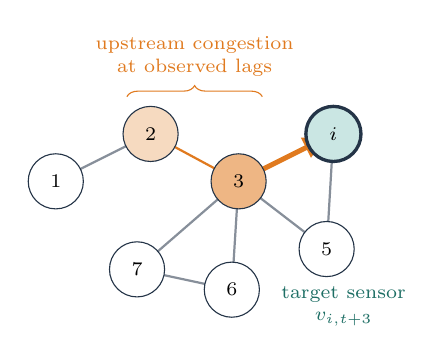
\begin{tikzpicture}[
      scale=0.86,
      sensor/.style={circle, draw=ink, minimum size=7mm, font=\scriptsize,
        fill=white},
      edge/.style={->, >=Latex, line width=0.8pt, draw=ink!55},
    ]
      \coordinate (a) at (0,2.0);
      \coordinate (b) at (1.4,2.7);
      \coordinate (c) at (2.7,2.0);
      \coordinate (d) at (4.1,2.7);
      \coordinate (e) at (4.0,1.0);
      \coordinate (f) at (2.6,0.4);
      \coordinate (g) at (1.2,0.7);
      \draw[edge] (a) -- (b);
      \draw[edge, graphorange] (b) -- (c);
      \draw[edge, graphorange, line width=1.8pt] (c) -- (d);
      \draw[edge] (c) -- (e);
      \draw[edge] (g) -- (c);
      \draw[edge] (f) -- (c);
      \draw[edge] (e) -- (d);
      \draw[edge] (g) -- (f);
      \node[sensor] at (a) {$1$};
      \node[sensor, fill=graphorange!28] at (b) {$2$};
      \node[sensor, fill=graphorange!55] at (c) {$3$};
      \node[sensor, fill=locationgreen!25, line width=1.2pt] at (d) {$i$};
      \node[sensor] at (e) {$5$};
      \node[sensor] at (f) {$6$};
      \node[sensor] at (g) {$7$};
      \draw[decorate, decoration={brace, amplitude=4pt}, graphorange]
        (1.05,3.25) -- (3.05,3.25)
        node[midway, above=4pt, font=\scriptsize, align=center]
        {upstream congestion\\at observed lags};
      \node[font=\scriptsize, align=center, text=locationgreen!70!black]
        at (4.25,0.15) {target sensor\\$v_{i,t+3}$};
    \end{tikzpicture}
    \caption{Directed sensor graph.}
    \label{fig:traffic-graph}
  \end{subfigure}\hfill
  \begin{subfigure}[t]{0.48\linewidth}
    \centering
    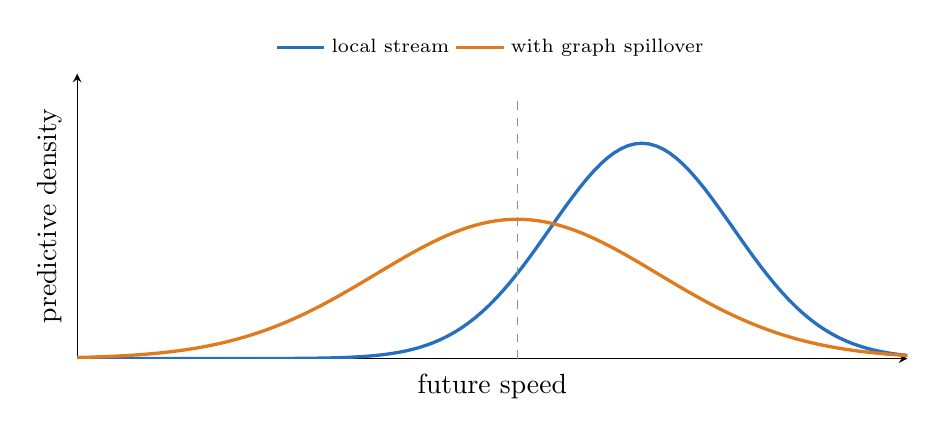
\begin{tikzpicture}
      \begin{axis}[
        width=\linewidth,
        height=52mm,
        axis lines=left,
        xlabel={future speed},
        ylabel={predictive density},
        xtick=\empty,
        ytick=\empty,
        xmin=0,xmax=10,ymin=0,ymax=0.48,
        legend style={draw=none,font=\scriptsize,at={(0.5,1.02)},
          anchor=south,legend columns=2},
      ]
        \addplot[localblue, very thick, domain=0:10, samples=120]
          {1/(1.1*sqrt(2*pi))*exp(-0.5*((x-6.8)/1.1)^2)};
        \addlegendentry{local stream}
        \addplot[graphorange, very thick, domain=0:10, samples=120]
          {1/(1.7*sqrt(2*pi))*exp(-0.5*((x-5.3)/1.7)^2)};
        \addlegendentry{with graph spillover}
        \draw[dashed, ink!55] (axis cs:5.3,0) -- (axis cs:5.3,0.44);
      \end{axis}
    \end{tikzpicture}
    \caption{Illustrative location and scale change.}
    \label{fig:traffic-density}
  \end{subfigure}
  \caption{Application schematic, not empirical results. Upstream congestion
  can shift the predicted location and increase conditional scale at a
  downstream sensor.}
  \label{fig:application}
\end{figure}

\subsection{Datasets and evaluation protocol}

\datasetA{} is the primary merit probe and \datasetB{} is the replication
dataset. Each dataset is split chronologically into 70\% training, 10\%
validation, and 20\% test blocks. Feature and target scalers are fitted on the
training block. Missing targets are masked; covariate imputation must use past
information only. The test block is evaluated once after model and stopping-rule
selection on validation data.

\section{Experiments}
\label{sec:experiments}

\subsection{Comparators and ablations}

\begin{table}[t]
  \centering
  \caption{Required comparisons and their scientific roles.}
  \label{tab:comparators}
  \begin{tabularx}{\linewidth}{lX}
    \toprule
    Model & Question answered\\
    \midrule
    Deterministic NAMLSS
      & Does graph information improve on local additive distributional regression?\\
    GAMLSS/BAMLSS
      & How does the neural local stream compare with established distributional regression?\\
    GAMLSS/BAMLSS + neighbor summaries
      & Is a learned graph representation better than simple graph covariates?\\
    Distributional GNN
      & Is the additive decomposition competitive with direct graph heads?\\
    Point GNN
      & Does distributional modeling seriously damage MAE or RMSE?\\
    \method{} ablations
      & Which distributional parameters and architecture factors use graph information?\\
    \bottomrule
  \end{tabularx}
\end{table}

The same-recipe comparison holds hidden dimensions and training settings fixed.
A second comparison approximately matches parameter counts. Required ablations
set the graph contribution to location only, scale only, both, and neither.

\subsection{Distributional metrics}

Let $z_{it}=(y_{it}-\mu_{it})/\sigma_{it}$, $\phi$ and $\Phi$ denote the
standard Normal density and CDF, and $\gamma$ the nominal interval level.
Besides \cref{eq:nll}, report
\begin{align}
  \crps\!\left(\mathcal{N}(\mu,\sigma^2),y\right)
    &=
    \sigma\left[
      z(2\Phi(z)-1)+2\phi(z)-\frac{1}{\sqrt{\pi}}
    \right],                                                        \label{eq:crps}\\
  u_{it}
    &= \Phi(z_{it}),                                                 \label{eq:pit}\\
  \widehat{\operatorname{Cov}}_{\gamma}
    &=
    \frac{1}{n_{\mathrm{test}}}
    \sum_{(i,t)\in\mathcal{T}_{\mathrm{test}}}
    \mathbb{1}\!\left\{
      q_{(1-\gamma)/2,it}\le y_{it}\le q_{(1+\gamma)/2,it}
    \right\}.                                                       \label{eq:coverage}
\end{align}
NLL and CRPS are proper scoring rules \citep{gneiting2007scoring}. MAE and RMSE
are point-accuracy guardrails.

\subsection{Interpretability outputs}

For every fitted model, retain:
\begin{equation}
  \left\{
    \widetilde f_{kj}(x),\;
    \alpha_k\widetilde r_{k,it},\;
    \alpha_k,\;
    \eta_{k,it}
  \right\}
  \quad
  \text{for }k\in\{\mu,\sigma\}.
  \label{eq:interpretability-artifacts}
\end{equation}
Plot local shapes with common feature grids, map graph contributions by sensor,
and display their temporal distributions. These are model diagnostics, not
causal explanations.

\begin{figure}[t]
  \centering
  \begin{subfigure}[t]{0.49\linewidth}
    \centering
    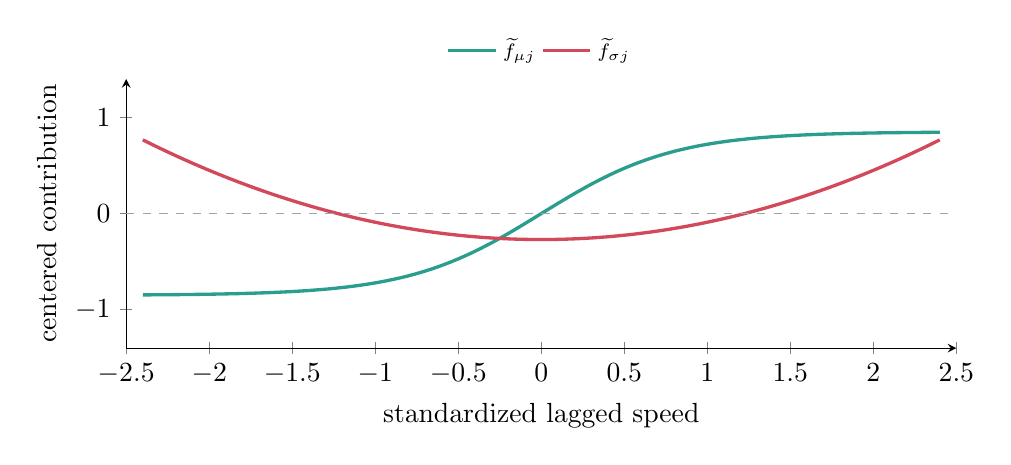
\begin{tikzpicture}
      \begin{axis}[
        width=\linewidth,height=50mm,
        axis lines=left,
        xlabel={standardized lagged speed},
        ylabel={centered contribution},
        xmin=-2.5,xmax=2.5,ymin=-1.4,ymax=1.4,
        legend style={draw=none,font=\scriptsize,at={(0.5,1.02)},
          anchor=south,legend columns=2},
      ]
        \addplot[locationgreen, very thick, domain=-2.4:2.4, samples=100]
          {0.85*tanh(1.25*x)};
        \addlegendentry{$\widetilde f_{\mu j}$}
        \addplot[scalered, very thick, domain=-2.4:2.4, samples=100]
          {0.18*x^2-0.27};
        \addlegendentry{$\widetilde f_{\sigma j}$}
        \addplot[ink!45,dashed] coordinates {(-2.5,0) (2.5,0)};
      \end{axis}
    \end{tikzpicture}
    \caption{Local shape-function template.}
  \end{subfigure}\hfill
  \begin{subfigure}[t]{0.49\linewidth}
    \centering
    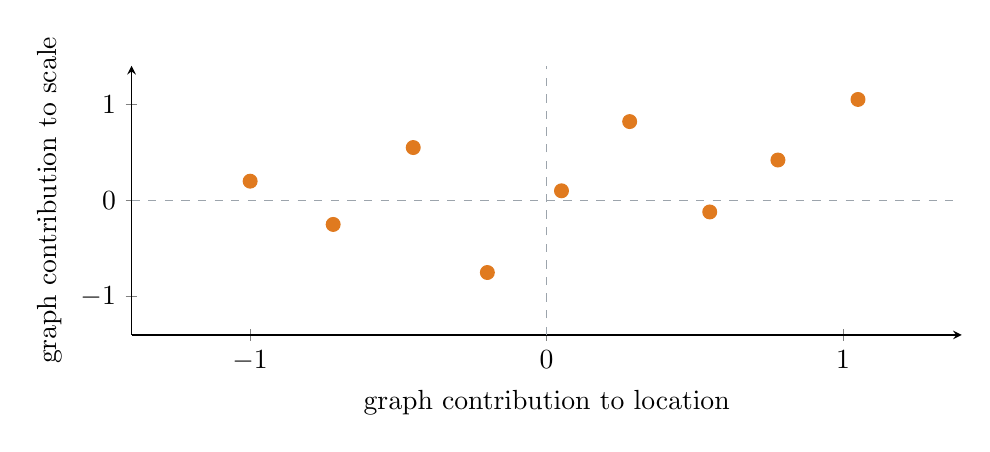
\begin{tikzpicture}
      \begin{axis}[
        width=\linewidth,height=50mm,
        axis lines=left,
        xlabel={graph contribution to location},
        ylabel={graph contribution to scale},
        xmin=-1.4,xmax=1.4,ymin=-1.4,ymax=1.4,
        xtick={-1,0,1},ytick={-1,0,1},
      ]
        \addplot[only marks, mark=*, mark size=2.5pt, graphorange]
          coordinates {
            (-1.0,0.20) (-0.72,-0.25) (-0.45,0.55) (-0.20,-0.75)
            (0.05,0.10) (0.28,0.82) (0.55,-0.12) (0.78,0.42) (1.05,1.05)
          };
        \addplot[ink!45,dashed] coordinates {(-1.4,0) (1.4,0)};
        \addplot[ink!45,dashed] coordinates {(0,-1.4) (0,1.4)};
      \end{axis}
    \end{tikzpicture}
    \caption{Graph-contribution diagnostic template.}
  \end{subfigure}
  \caption{Illustrative plot grammar. Replace coordinates with held-out model
  artifacts; do not retain the illustrative values in a submission.}
  \label{fig:interpretability}
\end{figure}

\subsection{Implementation and reproducibility}

Report software versions, random seeds, optimizer, learning-rate schedule,
batching, early stopping, graph direction, edge-weight handling, scaling
statistics, missingness rates, and total trainable parameters. The publication
candidate must be optimizer-trained using \cref{eq:nll}; the repository's
deterministic concept demonstrator is a pipeline and interpretability check, not
real-data evidence.

\section{Results}
\label{sec:results}

\subsection{Primary merit probe}

\begin{table}[t]
  \centering
  \caption{\datasetA{} test results. Lower is better for NLL, CRPS, MAE, and
  RMSE. Coverage should be interpreted relative to its nominal level.}
  \label{tab:primary-results}
  \sisetup{table-format=2.3}
  \begin{tabular}{l@{\hspace{4mm}}SSSSS}
    \toprule
    Model & {NLL} & {CRPS} & {Coverage} & {MAE} & {RMSE}\\
    \midrule
    NAMLSS                    & {--} & {--} & {--} & {--} & {--}\\
    NAMLSS + neighbor summary & {--} & {--} & {--} & {--} & {--}\\
    Distributional GNN        & {--} & {--} & {--} & {--} & {--}\\
    \method                   & {--} & {--} & {--} & {--} & {--}\\
    \bottomrule
  \end{tabular}
\end{table}

\placeholder{State the direction and uncertainty of the primary comparison.
Do not use the synthetic concept-demo metrics here.}

\subsection{Parameter-specific graph effects}

\begin{table}[t]
  \centering
  \caption{Graph-contribution ablation on \datasetA{}.}
  \label{tab:ablation-results}
  \begin{tabular}{lcccc}
    \toprule
    Graph contribution & NLL & CRPS & Coverage & RMSE\\
    \midrule
    none                  & -- & -- & -- & --\\
    location only         & -- & -- & -- & --\\
    scale only            & -- & -- & -- & --\\
    location and scale    & -- & -- & -- & --\\
    \bottomrule
  \end{tabular}
\end{table}

\placeholder{Summarize whether graph information acts mainly through location,
scale, or both. Report confidence intervals or repeated-run variation.}

\subsection{Replication and calibration}

\placeholder{Insert \datasetB{} replication table, PIT histograms, reliability
plots, and interval-width diagnostics after the primary merit probe passes.}

\section{Discussion}
\label{sec:discussion}

\placeholder{Interpret the primary distributional result and the local/graph
decomposition in two short paragraphs.}
The model provides conditional marginal distributions; it does not by itself
specify a joint predictive distribution over all sensors. Gate values and graph
maps are associational diagnostics. Results may depend on the supplied topology,
forecast horizon, missingness process, and Normal family.

\section{Conclusion}
\label{sec:conclusion}

\method{} offers a direct decomposition of local and graph-derived contributions
to multiple distributional parameters.
\placeholder{Add one sentence stating what the experiments established.}

\section*{Data and code availability}

\placeholder{Repository URL, release tag, dataset acquisition instructions, and
artifact DOI.}

\section*{Acknowledgements}

\placeholder{Funding, compute, and contributor acknowledgements.}

\bibliographystyle{plainnat}
\bibliography{references}

\appendix

\section{Notation}

\begin{table}[h]
  \centering
  \caption{Core notation.}
  \begin{tabularx}{\linewidth}{lX}
    \toprule
    Symbol & Meaning\\
    \midrule
    $\graph=(\mathcal{V},\mathcal{E},\bm{A})$ & directed weighted graph\\
    $\bm{x}_{it}$ & local covariates at node $i$, time $t$\\
    $\bm{z}_{it}$ & graph-stream covariates\\
    $f_{kj}$ & local shape function for parameter $k$, feature $j$\\
    $\bm{h}^{(L)}_{it}$ & final graph embedding\\
    $\widetilde r_{k,it}$ & centered graph-head output\\
    $\alpha_k$ & parameter-specific graph gate\\
    $\eta_{k,it}$ & additive predictor before inverse link\\
    $o_{it}$ & observed-target indicator\\
    \bottomrule
  \end{tabularx}
\end{table}

\section{Minimum reporting checklist}

\begin{enumerate}
  \item Confirm chronological splitting and train-only preprocessing.
  \item Separate concept-demonstrator results from merit-probe evidence.
  \item Report same-recipe and parameter-matched comparisons.
  \item Include location-only, scale-only, both, and no-graph ablations.
  \item Report NLL, CRPS, interval coverage, PIT, MAE, and RMSE.
  \item Archive local shapes, graph contributions, gates, and resolved configs.
  \item State whether the graph is directed and whether edge weights are used.
  \item Report repeated-run variation and the model-selection rule.
\end{enumerate}

\end{document}
